\documentclass[10pt]{article}
\usepackage[verbose, a4paper, hmargin=2.5cm, vmargin=2.5cm]{geometry}

\usepackage{fontspec}
\usepackage{ctex}
\usepackage{paratype}

\usepackage{amsmath}
\usepackage{amssymb}
\usepackage{amsfonts}
\usepackage{esint}
\usepackage{stmaryrd}

\usepackage[mathbf=sym]{unicode-math}
\setmainfont{STIX Two Text}
\setmathfont{STIX Two Math}

\setsansfont{Arial}
\setmonofont{Courier New}

\usepackage{makecell}
\usepackage{wasysym}
\usepackage{pifont}
\usepackage[export]{adjustbox}
\usepackage{graphicx}
\usepackage{mdframed}
\usepackage{booktabs,array,multirow}
\usepackage{tabularx}
\usepackage{hyperref}
\hypersetup{colorlinks=true, linkcolor=blue, filecolor=magenta, urlcolor=cyan,}
\urlstyle{same}
\usepackage[most]{tcolorbox}
\definecolor{mygray}{RGB}{240,240,240}
\tcbset{
  colback=mygray,
  boxrule=0pt,
}
\graphicspath{ {./images/} }
\newcommand{\HRule}{\begin{center}\rule{0.9\linewidth}{0.2mm}\end{center}}
\newcommand{\customfootnote}[1]{
  \let\thefootnote\relax\footnotetext{#1}
}
\newcommand{\lt}{\mathrel{<}}
\newcommand{\gt}{\mathrel{>}}
\newcommand*\circled[1]{\tikz[baseline=(char.base)]{\node[shape=circle,draw,inner sep=1.5pt] (char) {\small #1};}}
\setcounter{MaxMatrixCols}{256}
\begin{document}
\section*{2026 届上海市嘉定区高三数学二模}

\begin{center}

\includegraphics[max width=1.0\textwidth]{images/bo_d7ci95alb0pc73de9la0_0_0_1_1374_2337_0.jpg}
\end{center}
\hspace*{3em} 

\section*{一、填空题}

1. 已知集合 \(A = \left\{  {a,{a}^{2}}\right\}\) ，且 \(1 \in  A\) ，则 \(a =\) \_\_\_\_\_-1\_\_\_\_\_

\begin{center}
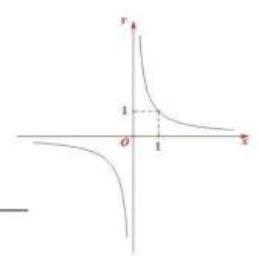
\includegraphics[max width=0.2\textwidth]{images/bo_d7ci95alb0pc73de9la0_1_765_504_259_256_0.jpg}
\end{center}
\hspace*{3em} 

\({a}^{2} = 1,\;a \neq  1\)

\(\therefore a =  - 1\)

2. 不等式 \(\frac{1}{x} > 1\) 的解集是\_\_\_\_\_ \(\left( {0,1}\right)\) \_\_\_\_\_

3. 已知角 \(\alpha\) 的终边经过点 \(P\left( {1, - 2}\right)\) ，则 \(\sin \alpha  =\) \_\_\_\_\_ \(- \frac{2\sqrt{5}}{5}\) \_\_\_\_\_

\(\sin \alpha  = \frac{y}{r} = \frac{-2}{\sqrt{5}} =  - \frac{2\sqrt{5}}{5}\)

4. 已知 \(\left\{  {a}_{n}\right\}\) 是等差数列， \({a}_{6} = 1,{a}_{26} = {11}\) ，则 \({a}_{2026} =\) \_\_\_\_\_1011\_\_\_\_\_

\({a}_{26} = {a}_{6} + {20d},\;{11} = 1 + {20d},\;d = \frac{1}{2}\)

\({a}_{2026} = {a}_{6} + {2020d} = 1 + {2020} \times  \frac{1}{2} = {1011}\)

5. 双曲线 \(\frac{{x}^{2}}{9} - \frac{{y}^{2}}{16} = 1\) 的渐近线方程为\_\_\_\_\_ \(y =  \pm  \frac{4}{3}x\) \_\_\_\_\_

6. 用 \(0\text{ 、 }1\text{ 、 }2\text{ 、 }3\text{ 、 }4\) 可以组成的没有重复数字的三位数的个数是\_\_\_\_\_48\_\_\_\_\_

\(4{P}_{4}^{2} = {48}\)

7. 函数 \(y = {\sin }^{4}x + {\cos }^{4}x\) 的最小正周期是\_\_\_\_\_ \(\frac{\pi }{2}\) \_\_\_\_\_

\(y = {\sin }^{4}x + {\cos }^{4}x = {\left( {\sin }^{2}x + {\cos }^{2}x\right) }^{2} - 2{\sin }^{2}x{\cos }^{2}x = 1 - 2{\left( \sin x\cos x\right) }^{2}\)

\(= 1 - 2{\left( \frac{1}{2}\sin 2x\right) }^{2} = 1 - \frac{1}{2}{\sin }^{2}{2x} = 1 - \frac{1}{2} \times  \frac{1 - \cos {4x}}{2}\)

\(T = \frac{2\pi }{4} = \frac{\pi }{2}\)

8. 已知函数 \(y = {x}^{3} + {x}^{2} + {ax}\) 有三个不同的零点,则实数 \(a\) 的取值范围是 \(\left( {-\infty ,0}\right)  \cup  \left( {0,\frac{1}{4}}\right)\)

\({x}^{3} + {x}^{2} + {ax} = 0,\;x\left( {{x}^{2} + x + a}\right)  = 0\)

\(x = 0\) 或 \({x}^{2} + x + a = 0\)

\(\left\{  \begin{array}{l} \Delta  = 1 - {4a} > 0 \\  a \neq  0 \end{array}\right.\)

\(\therefore a \in  \left( {-\infty ,0}\right)  \cup  \left( {0,\frac{1}{4}}\right)\)

9. 已知向量 \(\overrightarrow{a} = \left( {\cos x,\sin x}\right) ,\overrightarrow{b} = \left( {3,\sqrt{3}}\right)\) ，且 \(x \in  \left\lbrack  {0,\frac{\pi }{2}}\right\rbrack\) ，则 \(\overrightarrow{a}\) 在 \(\overrightarrow{b}\) 方向上的数量投影的取值范围

为 \(\left\lbrack  {\frac{1}{2},1}\right\rbrack\)

\begin{center}
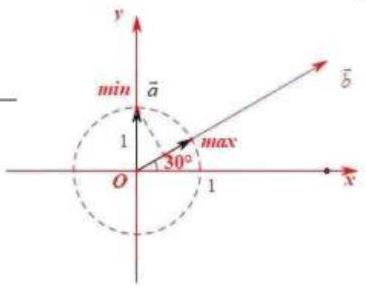
\includegraphics[max width=0.3\textwidth]{images/bo_d7ci95alb0pc73de9la0_2_470_745_366_288_0.jpg}
\end{center}
\hspace*{3em} 

10. 已知正四面体上的四个面上分别写有 \(1\text{ 、 }2\text{ 、 }3\text{ 、 }4\) ,游戏中甲、乙轮流抛掷该四面体,谁抛出底面数字等于 4 则获胜且游戏结束,甲先开始,则甲获胜的概率为\_\_\_\_\_ \(\frac{4}{7}\) \_\_\_\_\_

法一: 每次底面为 4 的概率为 \(\frac{1}{4}\)

\(P\left( \text{ 甲胜 }\right)  = \frac{1}{4} + \frac{3}{4} \times  \frac{3}{4} \times  \frac{1}{4} + \frac{3}{4} \times  \frac{3}{4} \times  \frac{3}{4} \times  \frac{3}{4} \times  \frac{1}{4} + \cdots\)

首项 \(\frac{1}{4},q = {\left( \frac{3}{4}\right) }^{2}\) 的无穷等比数列求和

\(S = \frac{\frac{1}{4}}{1 - {\left( \frac{3}{4}\right) }^{2}} = \frac{4}{7}\)

法二: 第二轮和第一轮甲先开始是等价的

\(P\left( \text{ 甲胜 }\right)  = \frac{1}{4} + \frac{3}{4} \times  \frac{3}{4}P\left( \text{ 甲胜 }\right)\)

\(P\left( \text{ 甲胜 }\right)  = \frac{4}{7}\)

11. 将函数 \(y = {x}^{2},x \in  \left\lbrack  {0,1}\right\rbrack\) 的图像绕坐标原点逆时针方向旋转角 \(\theta \left( {0 \leq  \theta  \leq  \alpha }\right)\) 得到曲线 \(\mathrm{C}\) ,若对于每一个角 \(\theta\) ,曲线 \(\mathrm{C}\) 都是一个函数的图像,则 \(\alpha\) 的最大值为\_\_\_\_\_ \(\arctan \frac{1}{2}\) \_\_\_\_\_

\(f\left( x\right)  = {x}^{2}\) ,在 \(x \in  \left\lbrack  {0,1}\right\rbrack\) 上任意两点的斜率 \(k = \frac{f\left( {x}_{1}\right)  - f\left( {x}_{2}\right) }{{x}_{1} - {x}_{2}} = \frac{{x}_{1}^{2} - {x}_{2}^{2}}{{x}_{1} - {x}_{2}} = {x}_{1} + {x}_{2} \in  \left\lbrack  {0,2}\right\rbrack \; \tan \theta  = 2\)

\begin{center}
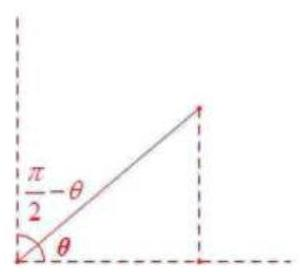
\includegraphics[max width=0.2\textwidth]{images/bo_d7ci95alb0pc73de9la0_3_843_348_301_272_0.jpg}
\end{center}
\hspace*{3em} 

最多旋转 \(\frac{\pi }{2} - \theta\) ,否则1个 \(x\) 对应 2 个 \(y\)

\(\tan \left( {\frac{\pi }{2} - \theta }\right)  = \frac{1}{\tan \theta } = \frac{1}{2}\)

\(\frac{\pi }{2} - \theta  = \arctan \frac{1}{2}\)

12. 在包装设计中,常用长度和宽度描述物体体型,长度 \(l\left( V\right)\) 定义为物体上最远两点间的距离, 宽度 \(t\left( V\right)\) 定义为能夹住物体的两平行平面间的最小距离,即存在一对平行平面,使得物体上的所有点均位于两平面之间 (包括平面上),现有一圆柱,其底面半径 \(\mathrm{R}\) 与高 \(\mathrm{h}\) 可任意调节,则 \(\frac{l\left( V\right) }{t\left( V\right) }\) 的最小值为\_\_\_\_\_ \(\sqrt{2}\) \_\_\_\_\_

\(l\left( V\right)  = \sqrt{{h}^{2} + {\left( 2R\right) }^{2}} = \sqrt{{h}^{2} + 4{R}^{2}}\)

\(t\left( V\right)\) 为能夹住该圆柱的两平行面间的最小距离,即该圆柱在任意直线上投影长度的最小值, 易知水平或竖直投影最小

\(t\left( V\right)  = \min \{ h,{2R}\}\)

\begin{center}
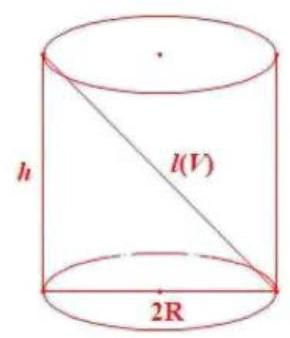
\includegraphics[max width=0.2\textwidth]{images/bo_d7ci95alb0pc73de9la0_3_968_1372_290_338_0.jpg}
\end{center}
\hspace*{3em} 

 \circled{1}  \(h \geq  {2R}\)

\(\frac{l\left( V\right) }{t\left( V\right) } = \frac{\sqrt{{h}^{2} + 4{R}^{2}}}{2R} = \sqrt{\frac{{h}^{2}}{4{R}^{2}} + 1} \geq  \sqrt{\frac{4{R}^{2}}{4{R}^{2}} + 1} = \sqrt{2}\)

 \circled{2}  \(h < {2R}\)

\(\frac{l\left( V\right) }{t\left( V\right) } = \frac{\sqrt{{h}^{2} + 4{R}^{2}}}{h} = \sqrt{1 + \frac{4{R}^{2}}{{h}^{2}}} > \sqrt{1 + \frac{4{R}^{2}}{4{R}^{2}}} = \sqrt{2}\)

综上， \(\min  = \sqrt{2}\)

\section*{二、选择题}

13. 已知陈述句 \(\alpha\) 是 \(\beta\) 的充分非必要条件,若集合 \(M = \{ x \mid  x\) 满足 \(\alpha \} ,\;N = \{ x \mid  x\) 满足 \(\beta \}\) ,则 \(M\) 与 \(N\) 的关系为 \(\left( A\right)\)

A. \(M \subset  N\) B. \(M \supset  N\) C. \(M = N\) D. \(M \cap  N = \varnothing\)

\(\alpha  \supsetneqq  \beta\) ,小 \(\Rightarrow\) 大,选 A

14. 生物学家在研究动物体重 \(\mathrm{W}\) (单位: \(\mathrm{g}\) ) 与脉搏率 \(f\) (单位: \(\mathrm{\text{ 次 }} \cdot  {\mathrm{{min}}}^{-1}\) ) 的关系时,获得了下表的数据,令 \(x = \ln W,y = \ln f\) ,并拟合线性回归方程 \(\widehat{y} = \widehat{a}x + \widehat{b}\) ,根据已知数据,下列说法正确的是(D)

\begin{center}
\adjustbox{max width=\textwidth}{
\begin{tabular}{|c|c|c|}
\hline
动物名 & 体重 W/(g) & 脉搏率 \(f/\left( {\text{ 次 } \cdot  {\mathrm{{min}}}^{-1}}\right)\) \\
\cline{1-3}
鼠 & 25 & 670 \\
\cline{1-3}
豚鼠 & 300 & 300 \\
\cline{1-3}
兔 & 2000 & 205 \\
\cline{1-3}
小狗 & 5000 & 120 \\
\cline{1-3}
大狗 & 30000 & 85 \\
\cline{1-3}
羊 & 50000 & 70 \\
\cline{1-3}
马 & 450000 & 38 \\
\cline{1-3}
\hline
\end{tabular}
}
\end{center}

A. 变量 \(x\) 与 \(\mathrm{y}\) 成正相关,且 \(\widehat{b} > 0\) B. 变量 \(x\) 与 \(\mathrm{y}\) 成负相关,且 \(\widehat{b} < 0\)

C. 变量 \(x\) 与 \(\mathrm{y}\) 成正相关,且 \(\widehat{b} < 0\) D. 变量 \(x\) 与 \(\mathrm{y}\) 成负相关,且 \(\widehat{b} > 0\)

15. 设数列 \(\left\{  {a}_{n}\right\}\) 满足 \({a}_{1} = 1\) ,且 \({a}_{n + 1} = \frac{\left( {{\lambda n} - 2}\right)  \cdot  {a}_{n}}{{n}^{2} + 1}\) ,其中 \(\lambda  \in  R\) ,下列选项中错误的是(C)

A. 存在 \(\lambda\) ,使得存在正整数 \(\mathrm{N}\) ,当 \(n \geq  N\) 时,总有 \({a}_{n + 1} < {a}_{n}\)

B. 存在 \(\lambda\) ,使得不存在正整数 \(\mathrm{N}\) ,当 \(n \geq  N\) 时,总有 \({a}_{n + 1} > {a}_{n}\)

C. 对任意 \(\lambda\) ,都不存在正整数 \(\mathrm{N}\) ,使得当 \(n \geq  N\) 时,总有 \({a}_{n + 1} > {a}_{n}\)

D. 存在 \(\lambda\) ,使得不存在正整数 \(\mathrm{N}\) ,当 \(n \geq  N\) 时,总有 \({a}_{n + 1} < {a}_{n}\)

当 \(\lambda  = 0\) 时, \({a}_{n + 1} = \frac{-2}{{n}^{2} + 1}{a}_{n},{a}_{1} = 1\)

\({a}_{n}\) 正负交替, \(\mathrm{B}\text{ 、 }\mathrm{D}\) 正确

当 \(\lambda  > 1\) 时, \({a}_{n + 1} = \frac{{\lambda n} - 2}{{n}^{2} + 1}{a}_{n} > 0,{a}_{1} = 1\)

当 \(n \rightarrow   + \infty\) 时, \({n}^{2} + 1 > {\lambda n} - 2,\frac{{\lambda n} - 2}{{n}^{2} + 1} < 1\)

\(\therefore \exists N\) ,当 \(n > N\) 时, \({a}_{n + 1} < {a}_{n},\mathrm{\;A}\) 正确

对于 \(\mathrm{C}\) ,尝试让 \({a}_{n}\left( {n \geq  2}\right)\) 为负, \(\frac{{\lambda n} - 2}{{n}^{2} + 1}\) 为 0 到1之间的正数

当 \(\lambda  = \frac{3}{2}\) 时, \({a}_{2} = \frac{\frac{3}{2} - 2}{1 + 1} =  - \frac{1}{4}\)

当 \(n \geq  2\) 时, \({n}^{2} + 1 > \frac{3}{2}n - 2,\frac{\frac{3}{2}n - 2}{{n}^{2} + 1} \in  \left( {0,1}\right)\)

\(\therefore\) 当 \(n \geq  2\) 时, \({a}_{n + 1} > {a}_{n},\mathrm{C}\) 错误,选 \(\mathrm{C}\)

16. 对任意平面向量 \(\overrightarrow{a},\overrightarrow{b},\overrightarrow{c}\) 及任意实数 \(\lambda\) ，已知运算 \(\odot\) 满足以下三条性质:

(I) \(\overrightarrow{a} \odot  \overrightarrow{b} = \overrightarrow{b} \odot  \overrightarrow{a}\) (II) \(\left( {\overrightarrow{a} + \overrightarrow{b}}\right)  \odot  \overrightarrow{c} = \overrightarrow{a} \odot  \overrightarrow{c} + \overrightarrow{b} \odot  \overrightarrow{c}\) (III) \(\left( {\lambda \overrightarrow{a}}\right)  \odot  \overrightarrow{b} = \lambda \left( {\overrightarrow{a} \odot  \overrightarrow{b}}\right)\) ,则下列选项中一定成立的是 \(\left( \begin{array}{ll} \mathrm{C} &  \end{array}\right)\)

A. 若 \(\overrightarrow{a} \odot  \overrightarrow{b} = 0\) ,则 \(\overrightarrow{a} = \overrightarrow{0}\) 或 \(\overrightarrow{b} = \overrightarrow{0}\) B. \(\left| {\overrightarrow{a} \odot  \overrightarrow{b}}\right|  = \left| \overrightarrow{a}\right|  \cdot  \left| \overrightarrow{b}\right|\)

C. \(\left( {\overrightarrow{a} - \overrightarrow{b}}\right)  \odot  \left( {\overrightarrow{a} - \overrightarrow{b}}\right)  = \overrightarrow{a} \odot  \overrightarrow{a} - 2\overrightarrow{a} \odot  \overrightarrow{b} + \overrightarrow{b} \odot  \overrightarrow{b}\) D. \(\overrightarrow{a} \odot  \overrightarrow{a} \geq  0\)

对于 \(\mathrm{A}\text{ 、 }\mathrm{\;B}\) ,可定义 \(\overrightarrow{a} \odot  \overrightarrow{b} = \overrightarrow{a} \cdot  \overrightarrow{b},\mathrm{\;A}\text{ 、 }\mathrm{\;B}\) 错误

对于 \(\mathrm{C}\) ,

\[
\left( {\overrightarrow{a} - \overrightarrow{b}}\right)  \odot  \left( {\overrightarrow{a} - \overrightarrow{b}}\right)  = \overrightarrow{a} \odot  \left( {\overrightarrow{a} - \overrightarrow{b}}\right)  + \left( {-\overrightarrow{b}}\right)  \odot  \left( {\overrightarrow{a} - \overrightarrow{b}}\right)
\]

\[
= \overrightarrow{a} \odot  \overrightarrow{a} + \overrightarrow{a} \odot  \left( {-\overrightarrow{b}}\right)  + \left( {-\overrightarrow{b}}\right)  \odot  \overrightarrow{a} + \left( {-\overrightarrow{b}}\right)  \odot  \left( {-\overrightarrow{b}}\right)
\]

\(= \overrightarrow{a} \odot  \overrightarrow{a} - \overrightarrow{a} \odot  \overrightarrow{b} - \overrightarrow{b} \odot  \overrightarrow{a} + \overrightarrow{b} \odot  \overrightarrow{b}\)

\(= \overrightarrow{a} \odot  \overrightarrow{a} - 2\overrightarrow{a} \odot  \overrightarrow{b} + \overrightarrow{b} \odot  \overrightarrow{b}\)

C 正确

对于 \(\mathrm{D}\) ,可定义 \(\overrightarrow{a} \odot  \overrightarrow{b} =  - \overrightarrow{a} \cdot  \overrightarrow{b}\) ,则 \(\overrightarrow{a} \odot  \overrightarrow{a} =  - {\left| \overrightarrow{a}\right| }^{2} \leq  0,\mathrm{D}\) 错误,选 \(\mathrm{C}\)

\section*{三、解答题}

17. 在复平面内,已知点 \(\mathrm{A}\text{ 、 }\mathrm{\;B}\text{ 、 }\mathrm{C}\) 对应的复数分别为 \({z}_{A} = 0,{z}_{B} = 6,{z}_{C} = 4 + 3\mathrm{i}\) ,其中 \(\mathrm{i}\) 是虚数单位.

(1)求 \(\cos \angle \mathrm{{ACB}}\) 的值；

(2)若复数 \(\mathrm{z}\) 满足 \(\left| {z - {z}_{A}}\right|  = \left| {z - {z}_{B}}\right|  = \left| {{z}_{B} - {z}_{C}}\right|\) ,求 \(\mathrm{z}\) .

(1) \(A\left( {0,0}\right) ,B\left( {6,0}\right) ,C\left( {4,3}\right)\)

\(\overrightarrow{CA} = \left( {-4, - 3}\right) ,\overrightarrow{CB} = \left( {2, - 3}\right)\)

\begin{center}
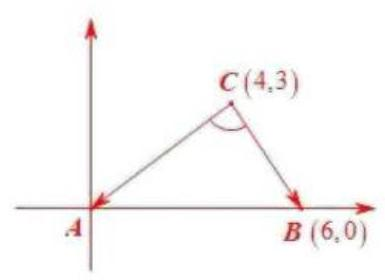
\includegraphics[max width=0.3\textwidth]{images/bo_d7ci95alb0pc73de9la0_6_964_294_385_280_0.jpg}
\end{center}
\hspace*{3em} 

\(\cos \angle {ACB} = \frac{\overrightarrow{CA} \cdot  \overrightarrow{CB}}{\left| \overrightarrow{CA}\right| \left| \overrightarrow{CB}\right| } = \frac{-4 \times  2 + \left( {-3}\right)  \times  \left( {-3}\right) }{5 \times  \sqrt{4 + 9}} = \frac{\sqrt{13}}{65}\)

(2)设 \(z = a + {bi}\)

\(\left| {z - {z}_{A}}\right|  = \sqrt{{a}^{2} + {b}^{2}},\;\left| {z - {z}_{B}}\right|  = \sqrt{{\left( a - 6\right) }^{2} + {b}^{2}}\)

\[
\left| {{z}_{B} - {z}_{C}}\right|  = \sqrt{4 + 9} = \sqrt{13}
\]

\(\left\{  \begin{array}{l} \sqrt{{a}^{2} + {b}^{2}} = \sqrt{13} \\  \sqrt{{\left( a - 6\right) }^{2} + {b}^{2}} = \sqrt{13} \end{array}\right.\) ,解得 \(\left\{  \begin{array}{l} a = 3 \\  b =  \pm  2 \end{array}\right.\)

\(\therefore z = 3 \pm  {2i}\)

18. 如图,在 \(\bigtriangleup  {ABC}\) 中， \(\angle \mathrm{{ACB}} = {90}^{ \circ  }\) ， \({DA} \bot\) 平面 \(\mathrm{{ABC}}\) ， \(\mathrm{M}\) 、 \(\mathrm{N}\) 分别是线段 \(\mathrm{{AC}}\) 、 \(\mathrm{{DB}}\) 的中点.

(1)求证: \({MN} \bot  {AC}\) ；

(2)若 \(\mathrm{{AC}} = \mathrm{{BC}} = \mathrm{{AD}} = 2\) ，求直线 \(\mathrm{{MN}}\) 与平面 \(\mathrm{{ABD}}\) 所成角的大小.

(1)取 \({AB}\) 中点 \(O\) ，连接 \({ON}\) 、 \({OM}\)

\begin{center}
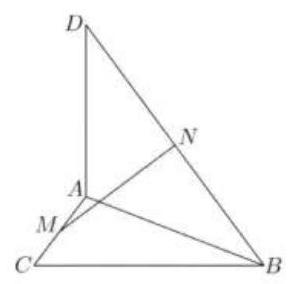
\includegraphics[max width=0.2\textwidth]{images/bo_d7ci95alb0pc73de9la0_6_978_1127_292_284_0.jpg}
\end{center}
\hspace*{3em} 

\(\because N\) 为 \({DB}\) 中点

\(\therefore {ON}\overset{//}{ = }\frac{1}{2}{AD}\)

\(\because {AD}\) 平面 \({ABC}\)

\(\therefore {ON} \bot\) 平面 \({ABC}\)

\begin{center}
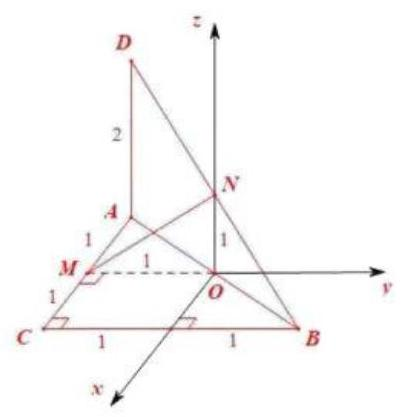
\includegraphics[max width=0.3\textwidth]{images/bo_d7ci95alb0pc73de9la0_6_906_1463_401_417_0.jpg}
\end{center}
\hspace*{3em} 

\(\therefore {MN}\) 在平面 \({ABC}\) 上的投影为 \({OM}\)

\(\because M\) 为 \({AC}\) 中点

\(\therefore {OM}\overset{//}{ = }\frac{1}{2}{BC}\)

\(\because \angle {ACB} = {90}^{ \circ  }\)

\(\therefore {OM} \bot  {AC}\)

\(\therefore {MN} \bot  {AC}\)

(2)如图建系， \(M\left( {0, - 1,0}\right)\) ， \(N\left( {0,0,1}\right)\) ， \(A\left( {-1, - 1,0}\right)\) ， \(B\left( {1,1,0}\right)\) ， \(D\left( {-1, - 1,2}\right) \; \overrightarrow{AB} = \left( {2,2,0}\right) ,\overrightarrow{AD} = \left( {0,0,2}\right) ,\overrightarrow{MN} = \left( {0,1,1}\right)\)

设平面 \({ABD}\) 的一个法向量为 \(\overrightarrow{n} = \left( {x,y,z}\right)\)

则 \(\left\{  \begin{array}{l} \overrightarrow{n} \cdot  \overrightarrow{AB} = {2x} + {2y} = 0 \\  \overrightarrow{n} \cdot  \overrightarrow{AD} = {2z} = 0 \end{array}\right.\) ,令 \(x = 1\) ,得 \(y =  - 1,z = 0,\overrightarrow{n} = \left( {1, - 1,0}\right)\)

\(\sin \theta  = \frac{\left| \overrightarrow{MN} \cdot  \overrightarrow{n}\right| }{\left| \overrightarrow{MN}\right| \left| \overrightarrow{n}\right| } = \frac{1}{\sqrt{2} \times  \sqrt{2}} = \frac{1}{2}\)

\(\therefore \theta  = \frac{\pi }{6}\)

19. 某款足球机器人射点球时,射门点与球门中心的水平偏差 (单位: \(\mathrm{{cm}}\) ) 服从正态分布,在正常状态下,偏差 \(\mathrm{X} \sim  \mathrm{N}\left( {0,{20}^{2}}\right)\) ,规定 \(\left| X\right|  > {60}\) 为“严重失误”.

(1)求一次射门出现严重失误的概率 \(\mathrm{p}\) (精确到 0.0001 )；

(2)假设每次射门相互独立，每次测试让机器人射门 16 次，若至少出现一次严重失误，则判定需要校准，在正常状态下，求一次测试被判定需要校准的概率 \(\alpha\) (精确到 0.01 )，并说明该判定规则是否合理；

(3)因机械磨损，机器人射门精度下降，一次射门出现严重失误的概率增加到 5\%，此时每次测试仍射门 16 次，但判定规则改为:若至少出现 2 次严重失误，才需要校准，在磨损状态下，求被判定需要校准的概率 \(\beta\) (精确到 0.01 )，此时，若一次校准的成本为 1 万元，且每天测试 3 次, 求日均校准成本的期望值 (精确到百元).

参考公式与数据:  \circled{1}  若 \(X \sim  N\left( {\mu ,{\sigma }^{2}}\right)\) ,则 \(Z = \frac{X - \mu }{\sigma } \sim  N\left( {0,1}\right)\)

 \circled{2}  若 \(Z \sim  N\left( {0,1}\right)\) ,则 \(P\left( {Z > 3}\right)  \approx  {0.00135},P\left( {Z > 2}\right)  \approx  {0.0228}\) .

(1) \(X \sim  N\left( {0,{20}^{2}}\right) ,\mu  = 0,\sigma  = {20}\)

\begin{center}
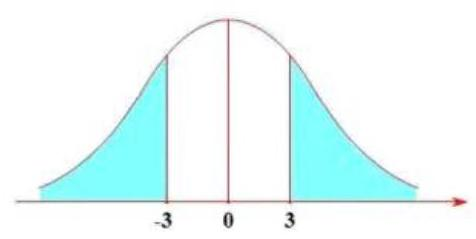
\includegraphics[max width=0.4\textwidth]{images/bo_d7ci95alb0pc73de9la0_7_844_1621_476_239_0.jpg}
\end{center}
\hspace*{3em} 

\(Z = \frac{X - \mu }{\sigma } \sim  N\left( {0,1}\right)\) ,即 \(Z = \frac{X}{20} \sim  N\left( {0,1}\right)\)

\(\left| X\right|  > {60},\;X \in  \left( {-\infty ,{60}}\right)  \cup  \left( {{60}, + \infty }\right)\)

\(Z = \frac{X}{20} \in  \left( {-\infty , - 3}\right)  \cup  \left( {3, + \infty }\right)\)

\(P = {2P}\left( {Z > 3}\right)  = 2 \times  {0.00135} = {0.0027}\)

(2)失误次数记为 \(Y\)

\[
P\left( {Y = 0}\right)  = {\left( 1 - {0.027}\right) }^{16}
\]

\(\alpha  = 1 - {\left( 1 - {0.0027}\right) }^{16} \approx  {0.04}\)

校准的概率较低, 花费少, 合理

(3) \(P\left( \text{ 失误 }\right)  = 5\%\)

\(\beta  = P\left( {Y \geq  2}\right)  = 1 - P\left( {Y = 0}\right)  - P\left( {Y = 1}\right)  = 1 - {\left( 1 - 5\% \right) }^{16} - {C}_{16}^{1}{\left( 1 - 5\% \right) }^{15}{\left( 5\% \right) }^{1} \approx  {0.19}\)

校准次数 \(\sim  B\left( {3,{0.19}}\right)\)

校准次数的期望为 \(3 \times  {0.19} = {0.57}\)

日均校准费用为 \({10000} \times  {0.57} = {5700}\) 元

20. 已知椭圆 \(\Gamma  : \frac{{x}^{2}}{{a}^{2}} + \frac{{y}^{2}}{4} = 1\left( {a > 2}\right)\) 与直线 \({l}_{1} : y = \frac{x}{2},{l}_{2} : y =  - \frac{x}{2}\) 过椭圆上一点 \(\mathrm{P}\) 作 \({l}_{1}\) 的平行线交 \({l}_{2}\) 于点 \(\mathrm{M}\) ,作 \({l}_{2}\) 的平行线交 \({l}_{1}\) 于点 \(\mathrm{N}\) .

(1)当 \(\mathrm{P}\) 为椭圆的上顶点时,求 \(\left| {MN}\right|\) 的大小;

(2)若椭圆的离心率 \(e = \frac{\sqrt{3}}{2}\) ，求椭圆 \(\Gamma\) 的方程，并求 \(\left| {\overrightarrow{OM} + \overrightarrow{ON}}\right|\) 的最大值与最小值；

(3)若 \(\left| {MN}\right|\) 为定值(与点 \(\mathrm{P}\) 的位置无关)，求 \(a\) 的值，并求此时四边形 ONPM 面积的最大值.

(1) \({PM} : y = \frac{1}{2}x + 2\) ，联立 \(y =  - \frac{1}{2}x\) ，得 \(M\left( {-2,1}\right)\)

\({PN} : y =  - \frac{1}{2}x + 2\) ,联立 \(y = \frac{1}{2}x\) ,得 \(N\left( {2,1}\right)\)

\begin{center}
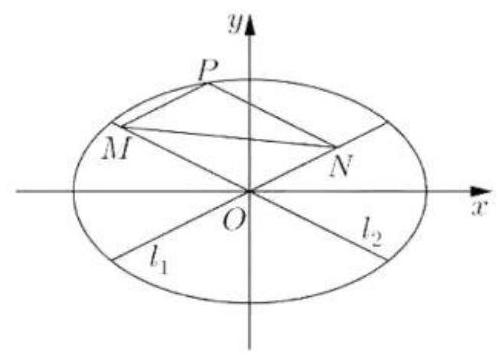
\includegraphics[max width=0.4\textwidth]{images/bo_d7ci95alb0pc73de9la0_8_902_1414_499_360_0.jpg}
\end{center}
\hspace*{3em} 

\(\therefore {MN} = 4\)

(2) \(\frac{c}{a} = \frac{\sqrt{3}}{2},b = 2,{a}^{2} = {b}^{2} + {c}^{2},a = 4 \; \therefore \Gamma  : \frac{{x}^{2}}{16} + \frac{{y}^{2}}{4} = 1\)

\(\because {PM}//{l}_{1},\because {PN}//{l}_{2}\)

\(\therefore\) 四边形 \({ONPM}\) 为平行四边形

设 \(P\left( {{x}_{0},{y}_{0}}\right)\) ,则 \(\frac{{x}_{0}{}^{2}}{16} + \frac{{y}_{0}{}^{2}}{4} = 1,{x}_{0}{}^{2} = {16} - 4{y}_{0}{}^{2}\)

\(\left| {\overrightarrow{OM} + \overrightarrow{ON}}\right|  = \left| \overrightarrow{OP}\right|  = \sqrt{{x}_{0}^{2} + {y}_{0}^{2}} = \sqrt{{16} - 4{y}_{0}^{2} + {y}_{0}^{2}} = \sqrt{{16} - 3{y}_{0}^{2}},\;{y}_{0} \in  \left\lbrack  {-2,2}\right\rbrack\)

\(\therefore {\left| \overrightarrow{OM} + \overrightarrow{ON}\right| }_{\max } = 4,{\left| \overrightarrow{OM} + \overrightarrow{ON}\right| }_{\min } = 2\)

(3) \({PM} : y - {y}_{0} = \frac{1}{2}\left( {x - {x}_{0}}\right)\) ，联立 \(y =  - \frac{1}{2}x\) ，得 \(M\left( {\frac{{x}_{0} - 2{y}_{0}}{2}, - \frac{{x}_{0} - 2{y}_{0}}{4}}\right)\)

\({PN} : y - {y}_{0} =  - \frac{1}{2}\left( {x - {x}_{0}}\right)\) ,联立 \(y = \frac{1}{2}x\) ,得 \(N\left( {\frac{{x}_{0} + 2{y}_{0}}{2},\frac{{x}_{0} + 2{y}_{0}}{4}}\right)\)

\(\therefore \overrightarrow{MN} = \left( {2{y}_{0},\frac{{x}_{0}}{2}}\right) ,\frac{{x}_{0}{}^{2}}{{a}^{2}} + \frac{{y}_{0}{}^{2}}{4} = 1,{y}_{0}{}^{2} = 4\left( {1 - \frac{{x}_{0}{}^{2}}{{a}^{2}}}\right)\)

\({\left| \overrightarrow{MN}\right| }^{2} = 4{y}_{0}{}^{2} + \frac{{x}_{0}{}^{2}}{4} = {16} - \frac{16}{{a}^{2}}{x}_{0}{}^{2} + \frac{{x}_{0}{}^{2}}{4} = {16} + \left( {\frac{1}{4} - \frac{16}{{a}^{2}}}\right)\)

\(\overrightarrow{MN}\) 为定值

\(\therefore \frac{16}{{a}^{2}} = \frac{1}{4},{a}^{2} = {64},a = 8,\frac{{x}_{0}^{2}}{64} + \frac{{y}_{0}^{2}}{4} = 1\)

\({S}_{\text{ 四 ONPM }} = \left| {{x}_{M} \cdot  {y}_{N} - {x}_{N} \cdot  {y}_{M}}\right|  = \left| \frac{{x}_{0}^{2} - 4{y}_{0}^{2}}{4}\right|  = \left| {{16} - 5{y}_{0}^{2}}\right| ,\;{y}_{0} \in  \left\lbrack  {-2,2}\right\rbrack\)

当 \({y}_{0} = 0\) 时, \({S}_{\max } = {16}\)

21. 已知在神经网络中, \(\sigma \left( x\right)  = \frac{1}{1 + {e}^{-x}}\) 常作为神经元激活函数.

(1)证明:对任意实数 \(x\) ，有 \(\sigma \left( {-x}\right)  + \sigma \left( x\right)  = 1\) ，并由此写出 \(y = \sigma \left( x\right)\) 图像的对称中心；

(2)设交叉熵损失函数 \({L}_{t}\left( y\right)  =  - \left\lbrack  {t\ln y + \left( {1 - t}\right) \ln \left( {1 - y}\right) }\right\rbrack\) ，用于衡量预测值 \(y\) 与真实标签 \(\mathrm{t}\) 之间的差异,其中 \(t \in  \{ 0,1\}\) ,试确定 \(\mathrm{t}\) 的值,使得 \(z = {L}_{t}\left( {\sigma \left( x\right) }\right)\) 在 \(\left( {-\infty , + \infty }\right)\) 上是减函数;

(3)在深度神经网络中，信号经过多层传播可抽象为一个迭代过程，设数列 \(\left\{  {x}_{n}\right\}\) 满足 \({x}_{n + 1} = \sigma \left( {x}_{n}\right)\) ,其中 \(\mathrm{n}\) 为正整数,证明: 存在唯一实数 \(A \in  \left( {0,1}\right)\) ,使得 \(\sigma \left( A\right)  = A\) ,且对任意实数 \({x}_{1}\) 和任意正整数 \(\mathrm{n}\) ,都有 \(\left| {{x}_{n + 2} - A}\right|  \leq  {\left( \frac{1}{4}\right) }^{n}\) .

(1) \(\sigma \left( {-x}\right)  + \sigma \left( x\right)  = \frac{1}{1 + {e}^{x}} + \frac{1}{1 + {e}^{-x}} = \frac{1}{1 + {e}^{x}} + \frac{{e}^{x}}{1 + {e}^{-x}} = 1\)

对称中心 \(\left( {0,\frac{1}{2}}\right)\)

(2)当 \(t = 0\) 时,

\({L}_{t}\left( {\sigma \left( x\right) }\right)  = \ln \left( {1 - \sigma \left( x\right) }\right)  =  - \ln \left( {1 - \frac{1}{1 + {e}^{-x}}}\right)  =  - \ln \left( \frac{1}{1 + {e}^{x}}\right)  = \ln \left( {1 + {e}^{x}}\right)\) 单调递增 (舍)

当 \(t = 1\) 时, \({L}_{t}\left( {\sigma \left( x\right) }\right)  =  - \ln \left( {\sigma \left( x\right) }\right)  =  - \ln \left( \frac{1}{1 + {e}^{-x}}\right)  = \ln \left( {1 + {e}^{-x}}\right)\) 单调递减

\(\therefore t = 1\)

(3)令 \(h\left( x\right)  = \sigma \left( x\right)  - x = \frac{1}{1 + {e}^{-x}} - x = 1 - \frac{1}{1 + {e}^{x}} - x\)

\({h}^{\prime }\left( x\right)  = \frac{{e}^{x}}{{\left( 1 + {e}^{x}\right) }^{2}} - 1 = \frac{{e}^{x}}{{e}^{2x} + 2{e}^{x} + 1} - 1 = \frac{1}{{e}^{x} + \frac{1}{{e}^{x}} + 2} - 1 \leq  \frac{1}{4} - 1 =  - \frac{3}{4} < 0\)

\begin{center}
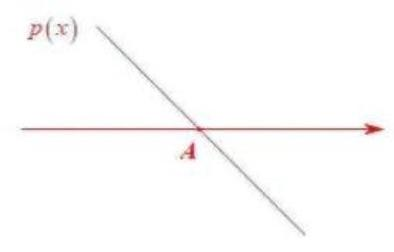
\includegraphics[max width=0.3\textwidth]{images/bo_d7ci95alb0pc73de9la0_10_1065_830_394_252_0.jpg}
\end{center}
\hspace*{3em} 

\(\therefore y = h\left( x\right)\) 单调递减

\(h\left( 0\right)  = \frac{1}{2},\;h\left( 1\right)  =  - \frac{1}{e + 1} < 0\)

\(\therefore\) 存在唯一 \(A \in  \left( {0,1}\right)\) ,使得 \(h\left( A\right)  = \sigma \left( A\right)  - A = 0\) ,即 \(\sigma \left( A\right)  = A\)

令 \(p\left( x\right)  = \sigma \left( x\right)  - A - \frac{1}{4}\left( {x - A}\right)\)

\begin{center}
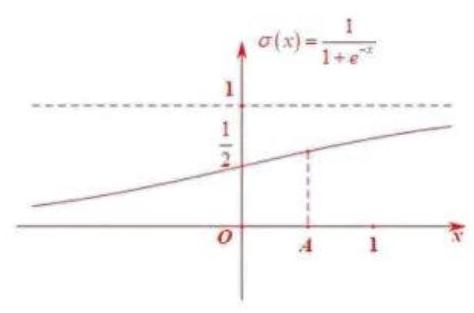
\includegraphics[max width=0.4\textwidth]{images/bo_d7ci95alb0pc73de9la0_10_979_1187_474_313_0.jpg}
\end{center}
\hspace*{3em} 

\({p}^{\prime }\left( x\right)  = {\sigma }^{\prime }\left( x\right)  - \frac{1}{4} \leq  0\)

\(\therefore y = p\left( x\right)\) 单调递减, \(p\left( A\right)  = \sigma \left( A\right)  - A = 0\)

当 \(x \geq  A\) 时, \(p\left( x\right)  \leq  0\) ,即 \(\sigma \left( x\right)  - A \leq  \frac{1}{4}\left( {x - A}\right)\)

当 \(x \leq  A\) 时, \(p\left( x\right)  \geq  0\) ,即 \(\sigma \left( x\right)  - A \geq  \frac{1}{4}\left( {x - A}\right)\)

\(\therefore \left| {\sigma \left( x\right)  - A}\right|  \leq  \frac{1}{4}\left| {x - A}\right|\) (实际拉格朗日中值定理)

\(\left| {{x}_{n + 2} - A}\right|  = \left| {\sigma \left( {x}_{n + 1}\right)  - A}\right|  \leq  \frac{1}{4}\left| {{x}_{n + 1} - A}\right|  = \frac{1}{4}\left| {\sigma \left( {x}_{n}\right)  - A}\right|  \leq  {\left( \frac{1}{4}\right) }^{2}\left| {{x}_{n - 1} - A}\right|  \leq  \cdots  \leq  {\left( \frac{1}{4}\right) }^{n}\left| {{x}_{2} - A}\right|\)

\[
{x}_{2} = \sigma \left( {x}_{1}\right)  \in  \left( {0,1}\right) ,\;A \in  \left( {0,1}\right)
\]

\[
\therefore \left| {{x}_{2} - A}\right|  < 1
\]

\(\therefore \left| {{x}_{n + 2} - A}\right|  < {\left( \frac{1}{4}\right) }^{n}\)

中国大陆 上海

\begin{center}

\includegraphics[max width=1.0\textwidth]{images/bo_d7ci95alb0pc73de9la0_11_53_481_1788_1824_0.jpg}
\end{center}
\hspace*{3em} 

\end{document}